

\usetikzlibrary{arrows.meta}

\definecolor{central}{RGB}{230,230,230}
\definecolor{rightc}{RGB}{66,133,244}
\definecolor{leftc}{RGB}{219,68,55}
\definecolor{topc}{RGB}{15,157,88}
\definecolor{bottomc}{RGB}{244,180,0}
\definecolor{goodball}{RGB}{88,86,214}
\definecolor{badball}{RGB}{171,71,188}

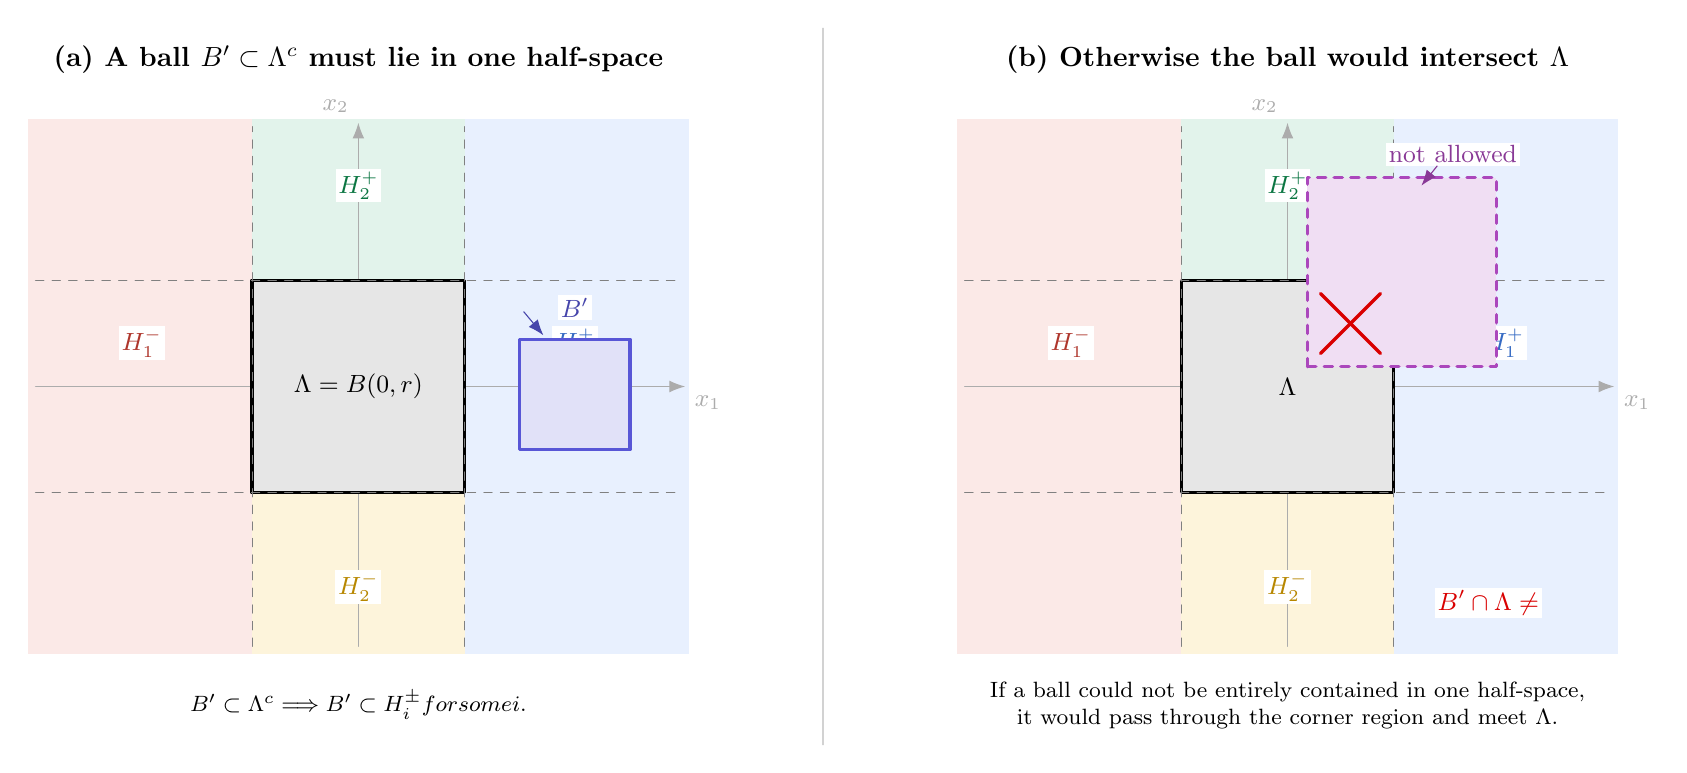
\begin{tikzpicture}[font=\small, line cap=round, line join=round]

% -------- Left panel: valid ball entirely in one half-space --------
\begin{scope}[shift={(-5.9,0)}]
  \node[font=\bfseries] at (0,4.15) {(a) A ball $B'\subset \Lambda^c$ must lie in one half-space};

  % half-space backgrounds
  \fill[rightc!12] (1.35,-3.4) rectangle (4.2,3.4);
  \fill[leftc!12]  (-4.2,-3.4) rectangle (-1.35,3.4);
  \fill[topc!12]   (-1.35,1.35) rectangle (1.35,3.4);
  \fill[bottomc!14](-1.35,-3.4) rectangle (1.35,-1.35);

  % coordinate axes
  \draw[-{Latex[length=2mm]},gray!65] (-4.1,0)--(4.15,0) node[below right] {$x_1$};
  \draw[-{Latex[length=2mm]},gray!65] (0,-3.3)--(0,3.35) node[above left] {$x_2$};

  % central region Lambda = B(0,r)
  \filldraw[fill=central,draw=black,very thick] (-1.35,-1.35) rectangle (1.35,1.35);
  \node[align=center] at (0,0) {$\Lambda=B(0,r)$};

  % guide lines
  \draw[dashed,gray] (-1.35,-3.3)--(-1.35,3.3);
  \draw[dashed,gray] (1.35,-3.3)--(1.35,3.3);
  \draw[dashed,gray] (-4.1,-1.35)--(4.1,-1.35);
  \draw[dashed,gray] (-4.1,1.35)--(4.1,1.35);

  % half-space labels
  \node[text=rightc!80!black,fill=white,inner sep=1pt] at (2.75,0.55) {$H_1^+$};
  \node[text=leftc!80!black,fill=white,inner sep=1pt] at (-2.75,0.55) {$H_1^-$};
  \node[text=topc!75!black,fill=white,inner sep=1pt] at (0,2.55) {$H_2^+$};
  \node[text=bottomc!75!black,fill=white,inner sep=1pt] at (0,-2.55) {$H_2^-$};

  % a valid l_infty-ball in the complement
  \filldraw[fill=goodball!18,draw=goodball,very thick]
    (2.05,-0.80) rectangle (3.45,0.60);
  \node[text=goodball!80!black,fill=white,inner sep=1pt] at (2.75,1.00) {$B'$};

  % statement arrow
  \draw[-{Latex[length=2mm]},goodball!80!black] (2.10,0.95)--(2.35,0.65);
  \node[align=center,font=\footnotesize] at (0,-4.05)
    {$B'\subset \Lambda^c\Longrightarrow B'\subset H_i^{\pm}\text{ for some }i.$};
\end{scope}

% -------- Right panel: straddling two half-spaces would hit Lambda --------
\begin{scope}[shift={(5.9,0)}]
  \node[font=\bfseries] at (0,4.15) {(b) Otherwise the ball would intersect $\Lambda$};

  % half-space backgrounds
  \fill[rightc!12] (1.35,-3.4) rectangle (4.2,3.4);
  \fill[leftc!12]  (-4.2,-3.4) rectangle (-1.35,3.4);
  \fill[topc!12]   (-1.35,1.35) rectangle (1.35,3.4);
  \fill[bottomc!14](-1.35,-3.4) rectangle (1.35,-1.35);

  % coordinate axes
  \draw[-{Latex[length=2mm]},gray!65] (-4.1,0)--(4.15,0) node[below right] {$x_1$};
  \draw[-{Latex[length=2mm]},gray!65] (0,-3.3)--(0,3.35) node[above left] {$x_2$};

  % central region
  \filldraw[fill=central,draw=black,very thick] (-1.35,-1.35) rectangle (1.35,1.35);
  \node[align=center] at (0,0) {$\Lambda$};

  % guide lines
  \draw[dashed,gray] (-1.35,-3.3)--(-1.35,3.3);
  \draw[dashed,gray] (1.35,-3.3)--(1.35,3.3);
  \draw[dashed,gray] (-4.1,-1.35)--(4.1,-1.35);
  \draw[dashed,gray] (-4.1,1.35)--(4.1,1.35);

  % half-space labels
  \node[text=rightc!80!black,fill=white,inner sep=1pt] at (2.75,0.55) {$H_1^+$};
  \node[text=leftc!80!black,fill=white,inner sep=1pt] at (-2.75,0.55) {$H_1^-$};
  \node[text=topc!75!black,fill=white,inner sep=1pt] at (0,2.55) {$H_2^+$};
  \node[text=bottomc!75!black,fill=white,inner sep=1pt] at (0,-2.55) {$H_2^-$};

  % a hypothetical bad ball that straddles two half-spaces and touches Lambda
  \filldraw[fill=badball!18,draw=badball,very thick,dashed]
    (0.25,0.25) rectangle (2.65,2.65);
  \node[text=badball!80!black,fill=white,inner sep=1pt] at (2.10,2.95) {not allowed};
  \draw[-{Latex[length=2mm]},badball!80!black] (1.90,2.80)--(1.70,2.55);

  % emphasize forbidden overlap
  \draw[red!85!black,very thick] (0.42,0.42)--(1.18,1.18);
  \draw[red!85!black,very thick] (0.42,1.18)--(1.18,0.42);
  \node[text=red!85!black,fill=white,inner sep=1pt] at (2.55,-2.75) {$B'\cap\Lambda\neq\varnothing$};

  \node[align=center,font=\footnotesize] at (0,-4.05)
    {If a ball could not be entirely contained in one half-space,\\
     it would pass through the corner region and meet $\Lambda$.};
\end{scope}

% separator
\draw[gray!35] (0,-4.55)--(0,4.55);

\end{tikzpicture}

